\documentclass[twoside]{article}

\usepackage{enumitem} % for customizing enumerate tags
\usepackage{amsmath,amsthm,amssymb}
\usepackage{listings}
\usepackage{subcaption}
\usepackage{minted}
\usepackage[math]{kurier}
\usepackage[sc]{mathpazo}
\renewcommand{\sfdefault}{kurier}


\usepackage{graphics}
\usepackage{graphicx}
\setlength{\oddsidemargin}{0.25 in}
\setlength{\evensidemargin}{-0.25 in}
\setlength{\topmargin}{-0.6 in}
\setlength{\textwidth}{6.5 in}
\setlength{\textheight}{8.5 in}
\setlength{\headsep}{0.75 in}
\setlength{\parindent}{0 in}
\setlength{\parskip}{0.1 in}

\newcounter{lecnum}
\renewcommand{\thepage}{\thelecnum-\arabic{page}}
\renewcommand{\thesection}{\thelecnum.\arabic{section}}
\renewcommand{\theequation}{\thelecnum.\arabic{equation}}
\renewcommand{\thefigure}{\thelecnum.\arabic{figure}}
\renewcommand{\thetable}{\thelecnum.\arabic{table}}




\newcommand{\lecture}[3]{
   \pagestyle{myheadings}
   \thispagestyle{plain}
   \newpage
   \setcounter{lecnum}{#1}
   \setcounter{page}{1}
   \noindent
   \begin{center}
   \framebox{
      \vbox{\vspace{2mm}
    \hbox to 6.28in { {\bf \sffamily AA 274: Principles of Robotic Autonomy
                        \hfill Winter 2018} }
       \vspace{4mm}
       \hbox to 6.28in { {\sffamily{\Large \hfill Lecture #1: #2  \hfill}} }
       \vspace{2mm}
       % \hbox to 6.28in { {\it \hfill Scribes: #4} }
      \vspace{2mm}}
   }
   \end{center}
   \markboth{Lecture #1: #2}{Lecture #1: #2}

   \vspace*{4mm}
}



%%%%%%%%%%%%%%%%%%%%%%%%%%
%document
\begin{document}
%modify this
\lecture{9}{Machine Learning and Modern Visual Recognition Techniques}{}


\section{Introduction}
This lecture provides an introduction to neural networks and proceeds to discuss Convolutional neural networks, which are especially suited to process images. With the advance of technology the amount of data available for any given task has gone up exponentially  in the last several decades. Methods such as logistic regression perform well when the training data set is large. But their performance plateaus out after a point. Neural networks have gained popularity because with huge amounts of data which is currently available, even small neural networks are able to outperform traditional learning algorithms by large margins. 

Image recognition and image processing has widespread applications in robotics such as  path identification, obstacle avoidance etc. If we were to use a standard neural network architecture to process images, we would need to learn parameters of the order of millions. Convolutional neural networks have significantly brought down this number by using special convolution layers which exploits the spatial structure of images. 

The core learning objectives of this lecture are:
\begin{enumerate}
     \item The basics of neural networks :
     \begin{itemize}
         \item How neural networks mimic the architecture of human brain and how multiple layers of the network work together
         \item How to train a Neural network to do a particular task and where they could go wrong
     \end{itemize}
     \item Convolutional neural networks:
     \begin{itemize}
         \item This section covers in depth the different elements of a Convolutional neural network and some famous architectures commonly used in the industry 
     \end{itemize}
 \end{enumerate}
 


\section{Neural Network Basics}
Work on Artificial neural networks, generally known as just 'neural networks', has been inspired by the fact that the human brain processes information in a completely different way than computers. Due to this, human brains are much more efficient at certain tasks, such as vision, language processing, etc. than computers. Artificial neural networks aim to mimic this biological model by employing a large number of simple interconnected processing units or 'neurons'.  We may thus offer the following definition of a neural network viewed as an adaptive machine\cite{haykin}:

A neural network is a massively parallel distributed processor made up of simple processing units that has a natural propensity for storing experiential knowledge and making it available for use. It resembles the brain in two respects:\\
1. Knowledge is acquired by the network from its environment through a learning process.\\
2. Inter-neuron connection strengths, known as synaptic weights, are used to store the acquired knowledge.

\subsection{Perceptron - Analogy to a Biological Neuron}
The figure below shows a simplified diagram of a biological neuron:

\begin{figure}[!htb]
\centering
\includegraphics[height = 2in]{pics/neuron.png}
\caption{Simplified model of a biological neuron\cite{cs231n-website}}
\label{fig:bio-neuron}
\end{figure}

There are approximately 86 billion neurons in the human nervous system and they are connected with approximately $10^{14}$ - $10^{15}$ synapses\cite{cs231n-website}.

The figure below shows a commonly used mathematical model of a neuron:

\begin{figure}[!htb]
\centering
\includegraphics[height = 2in]{pics/neuron_model.jpeg}
\caption{Mathematical model of a neuron\cite{cs231n-website}}
\label{fig:neuron_model}
\end{figure}

Signals travel along the axons (e.g. $x_0$) and interact multiplicatively (e.g. $w_{0}x_{0}$) with the dendrites of the other neuron based on the synaptic strength at that synapse (e.g. $w_0$). The idea is that the synaptic strengths (the weights $w$) are learnable and control the strength of influence (and its direction: excitatory (positive weight) or inhibitory (negative weight)) of one neuron on another. We can model the firing rate of the neuron with an activation function $f$, which represents the frequency of the spikes along the axon. Historically, a common choice of activation function was the sigmoid function, but the ReLU function is more commonly used nowadays. This is because the gradient of the sigmoid function becomes small as its value increases which reduces the training speed of the model.


\subsection{Single Layer Network / Logistic Regression}
Inspired by this model of the neuron, a single-layer neural net can be built which takes in binary inputs and provides binary output by taking a weighted sum and passing it through an activation function (as seen below). The theory is that if these weights are tuned perfectly, then it should be able to classify the inputs correctly.


\begin{figure}[!htb]
\centering
\includegraphics[height = 2in]{pics/Logistic_regression.png}
\caption{Single layer neural net\cite{Lecture slides}}
\label{fig:Single layer neural net}
\end{figure}


\subsection{Multi-layer Neural Network / Deep Learning}

We can get more resolution on our classifications by putting multiple of these layers together. In such regard, each layer can "learn" to classify a different part of the input. Take for an example the problem of classifying handwritten digits, in particular classifying the number 3. The first layer can be responsible for classifying a curved top, the second a curved bottom, etc.

A sample is shown below (from : http://www.cs.cmu.edu/~aharley/vis/conv/flat.html)

\begin{figure}[!htb]
\centering
\includegraphics[height = 2in]{pics/deep_neural_net.png}
\caption{Deep Neural Net for Classifying Handwritten Numbers\cite{}}
\label{fig:Single layer neural net}
\end{figure}

Representing this is simply a bunch of single layer neural networks linked together where the output of 1 layer is the input of the second layer.

\begin{figure}[!htb]
\centering
\includegraphics[height = 2in]{pics/deep_learning.png}
\caption{Deep Learning\cite{}}
\label{fig:Deep Learning}
\end{figure}

\subsection{Activation Functions}

If we didn't use non-linear activation functions, the output of the neural network would just be a linear function of the input. Such a network is basically just a Linear regression Model and and no matter how many layer and nodes we add to such a network, it is equivalent to having a network with a single node.\\

Hence, we use Activation functions to make the network more powerful give it the ability to represent non-linear complex functional mappings between inputs and outputs.

Another important feature of an Activation function is that it should be differentiable. This is because we perform back-propagation to calculate the gradients of the Loss function with respect to the weights and then accordingly optimize weights using gradient descend or any other Optimization technique to decrease the Loss Function.

The following are the most commonly used activation functions:

\begin{enumerate}

\item \textbf{Sigmoid Function:}
The Sigmoid Function takes a real-valued number and maps it to a range between 0 and 1.
\begin{figure}[!htb]
\centering
\includegraphics[height = 1.2in]{pics/sigmoid.jpeg}
\caption{The sigmoid function\cite{cs231n-website}}
\label{fig:sigmoid}
\end{figure}
\begin{equation*}
f(x) = \frac{1}{1+e^{-x}}
\end{equation*}
Sigmoid Activation functions have historically been used extensively but have now fallen out of favor due to the following drawbacks:
\begin{enumerate}
\item They are prone to saturate as the gradients are very small away from the center. When this occurs, almost no signal will flow through the neuron to its weights and recursively to its data.
\item They are not zero-centered.
\end{enumerate}

\item \textbf{Tanh function:}
The Tanh function looks quite similar to a sigmoid function. It maps a real-valued number to a range between -1 and 1.
\begin{figure}[!htb]
\centering
\includegraphics[height = 1.2in]{pics/tanh.jpeg}
\caption{The tanh function\cite{cs231n-website}}
\label{fig:tanh}
\end{figure}
\begin{equation*}
f(x) = \tanh(x)
\end{equation*}
It saturates in the same way as a sigmoid does but it has the advantage of being zero-centered. Hence, in practice, it is always preferred to a sigmoid function.

\item \textbf{ReLU Function:}
The Rectified Linear Unit is simply a threshold at zero and has become very popular in the last few years.
\begin{figure}[!htb]
\centering
\includegraphics[height = 1.2in]{pics/relu.jpeg}
\caption{The ReLU function\cite{cs231n-website}}
\label{fig:ReLU}
\end{figure}
\begin{equation*}
f(x) = max( 0, x )
\end{equation*}
It has the following advantages:
\begin{enumerate}
\item It greatly accelerates the convergence of stochastic gradient descent compared to tanh/sigmoid.
\item It is computationally cheaper to implement than tanh/sigmoid as it can implemented by simply thresholding a matrix of activations at zero.
\end{enumerate}
The main disadvantage of the ReLU is that ReLU units can irreversibly die during training since they can get knocked off the data manifold.

\item \textbf{Leaky ReLU Function:}
The Leaky ReLU attempts to fix the problem of dying nuerons by providing a small negative slope in the $x<0$ region.
\begin{figure}[!htb]
\centering
\includegraphics[height = 1.2in]{pics/Leaky.png}
\caption{The Leaky ReLU function\cite{cs231n-website}}
\label{fig:ReLU}
\end{figure}
\begin{equation*}
f(x) = max( 0.1 x, x )
\end{equation*}

\end{enumerate}
\subsection{Training Neural Networks}
We now need a way to teach these neural networks weights to make correct predictions. This is done by running the network on known data points and updating the weights of the neurons based on the correctness of the model in classifying the input. \\

Running this however on each input one at a time can take a long period of time for training. Instead these models are run on a sample batch of data. In particular the steps are the following.\\

\begin{figure}[!htb]
\centering
\includegraphics[height = 2in]{pics/training_net.png}
\caption{Training a neural net\cite{}}
\label{fig:Training a neural net}
\end{figure}

\textbf{1. Sample a batch of data.}
We can use a smaller batch of data at each iteration to train the model to decrease training time.

\textbf{2. Run the input it through the graph and compute the loss.}
The loss function provides serves as a quality metric and provides us an idea on the error of our model. That is, how correct it is.

\textbf{3. Backpropagate}
Activation functions are chosen to be differentiable to make this step easier. Backpropagation is done by taking the gradient with respect to the weights of each neuron in each layer.

\textbf{4. Update these parameters using SGD (Stochastic Gradient Descent)}
Update each parameter using the gradient calculated in the previous step

\textbf{5. Repeat many times}

\subsection{Overfitting}
Creating complex models sometimes have the disadvantage of being extremely accurate only on the test data. That is, the model is able to classify its entire training data with high accuracy however is unable to generalize and fails with test / real data.

On the other hand too simple models are unable to learn the more subtle trends in the data.

\begin{figure}[!htb]
\centering
\includegraphics[height = 2in]{pics/overfitting.png}
\caption{Overfitting\cite{}}
\label{fig:Overfitting}
\end{figure}
http://mlwiki.org/index.php/Overfitting

In the example above the left model was too simple and was unable to classify some of the values correctly. On the other the right model despite perfectly classifying on this training dataset is unlikely to perform as well in real-world situations. The middle offers a good classification.

To combat overfitting, regularizaiton is usually introduced in models. Regularization is a technique that penalizes complex models or prevents them from being made. Some of these techniques include

\textbf{Dropout}
Randomly select neurons that will not be activated at each pass during training.

\textbf{L2 Regularization}
Penalize the square magnitude of all parameters which forces neuron size to be smaller.

\textbf{Max Norm Constraints}
Limit the maximum weight of a neuron.


%%%%%%%%%%%%
% PART III %
%%%%%%%%%%%%
\section{Convolutional Neural Networks}
A simple Convolutional Neural Networks is a sequence of layers, and every layer of a Convolutional Neural Networks transforms one volume of activations to another through a differentiable function. There are four main types of layers to build ConvNet architectures: \textbf{Convolutional Layer}, \textbf{Nonlinearity Layer}, \textbf{Pooling Layer}, and \textbf{Fully-Connected Layer}. These layers are stacked to form a full ConvNet architecture. In this way, Convolutional Neural Networks transform the original image layer by layer from the original pixel values to the final class scores.

In this section, we mainly discuss the three types of layer in Convolutional Neural Networks, including Convolutional layer, Pooling layer and Fully-connected layer.

\subsection{Convolutional Layer}
\textbf{Parameter Sharing}
Parameter sharing scheme is used in Convolutional Layers to control the number of parameters. It is hard to make perceptrons scalable when the input image size is large given the fact the number of parameters grow quickly with the input size. However, we can dramatically reduce the number of parameters by making one reasonable assumption. If we know the input is image data, we can assume some spatial symmetries. In other word, if one feature is useful to compute at some spatial position $(x,y)$, then it should also be useful to compute at a different position $(x_2,y_2)$, so same parameters could be used.

\textbf{Convolution Details}
The convolution operation essentially performs dot products between the filters and local regions of the input. In other words, each element is computed by element-wise multiplying the local regions of the input (blue part in Figure \ref{fig:conv_demo}) with the filter (red part in Figure \ref{fig:conv_demo}), summing it up, and then offsetting the result by the bias. The output is the green part in Figure \ref{fig:conv_demo}.

Noticing we give the demo in 2D format. In real cases, the input would be a 3D tensor while he depth of the output volume is a hyperparameter. It corresponds to the number of filters we would like to use, each learning to look for something different in the input. Take Figure \ref{fig:conv_demo2} as an example, if we have 6 $5\times5$ filters, we will get 6 separate activation maps as output.

\textbf{Spatial arrangement} Besides depth, there are two hyperparameters to control the size of the output volume: the stride and zero-padding
\begin{itemize}
\item \textbf{stride} Stride specifies how we slide the filter. When the stride is 1 then we move the filters one pixel at a time. When the stride is 2 (or uncommonly 3 or more, though this is rare in practice) then the filters jump 2 pixels at a time as we slide them around.
\item \textbf{zero-padding} In some cases, the size of filters and stride don’t “fit” neatly and symmetrically across the input. For example, if the input size $H=W=10$ while the filter size is $F=3$ and it takes stride $S=3$, it would be impossible to use stride $S=2$, since
\begin{equation}
\begin{aligned}
(H-F)/S+1&=(10-3)/3+1=3.33~\text{(Not an integer)}\\
(W-F)/S+1&=(10-3)/3+1=3.33~\text{(Not an integer)}\\
\end{aligned}
\end{equation}
Therefore, we need to use zero-padding. We add additional zero-paddings in the contour of the image. If we take zero-padding $P=1$, we would have
\begin{equation}
\begin{aligned}
(H-F+2*P)/S+1&=(10-3+2*1)/3+1=4~\text{(An integer)}\\
(W-F+2*P)/S+1&=(10-3+2*1)/3+1=4~\text{(An integer)}\\
\end{aligned}
\end{equation}
\end{itemize}

In general, setting zero padding to be $P=(F−1)/2$ when the stride is $S=1$ ensures that the input volume and output volume will have the same size spatially. It is very common to use zero-padding in this way.

\begin{figure}[!htb]
\centering
\includegraphics[height = 3in]{pics/cnn.png}
\caption{Convolution Demo\cite{cs231n-website}}
\label{fig:conv_demo}
\end{figure}

\begin{figure}[!htb]
\centering
\includegraphics[height = 2in]{pics/cnn2.png}
\caption{Number of filter and depth of output\cite{cs231n-website}}
\label{fig:conv_demo2}
\end{figure}
\subsection{Pooling Layer}
In practice, it is common to periodically insert a Pooling Layer in-between successive Conv layers in a ConvNet architecture. It is mainly used to progressively reduce the spatial size of the representation to reduce the amount of parameters and computation load, and hence to also control overfitting. The Pooling Layer operates independently on every depth slice of the input and resizes it spatially, using the MAX operation if max pooling, AVG if average pooling, etc. The most common form is a pooling layer with filters of size $2\times2$ applied with a stride of 2 downsamples every depth slice in the input by 2 along both width and height, discarding 75\% of the activations. In this case, every pooling operation would be taking a max or average over 4 numbers (little $2\times2$ region in some depth slice). The depth dimension remains unchanged. In a nutshell, \textit{pooling layer \textbf{downsamples} the volume spatially, independently in \textbf{each} depth slice of the input volume.}

\begin{figure}[!htb]
\begin{subfigure}[!htb]{0.45\linewidth}
\includegraphics[scale=0.33]{pics/pool}
\caption{general pooling}
\label{fig:genpool}
\end{subfigure}
\hfill
\begin{subfigure}[!htb]{0.54\linewidth}
\includegraphics[scale=0.33]{pics/maxpool}
\caption{max pooling}
\label{fig:maxpool}
\end{subfigure}
\caption{Pooling Layer\cite{cs231n-website}}
\end{figure}

The Fig.\ref{fig:genpool} shows how pooling works generally. A $2\times2$ pooling filter with stride 2 is applied on the $224\times224\times64$ input volume, yielding the $112\times112\times64$ output volume. Note that the width and height of the input volume shrinks to half while the depth is preserved. The most common downsampling operation is MAX. The Fig.\ref{fig:maxpool} here shows max pooling with a stride of 2. That is, each max is taken over 4 numbers in a $2\times2$ square. For instance, the top-left red square squashes to a single value, \texttt{\textbf{6}}, which is \texttt{\textbf{max\{1, 1, 5, 6\}}}.

\subsection{Fully-Connected Layer}
The last few layers of a ConvNet architecture are typically Fully-Connected (FC) Layers. As seen in regular neural networks, FC Layers serve as a linear classifier for classification or regression. Their activations can be computed with a matrix multiplication followed by a bias offset, \textit{i.e.} $f = Wx + b$. See the Neural Network Basics section of the note for more information.

\subsection{Mainstream Model Architectures}
\begin{figure}[!htb]
\centering
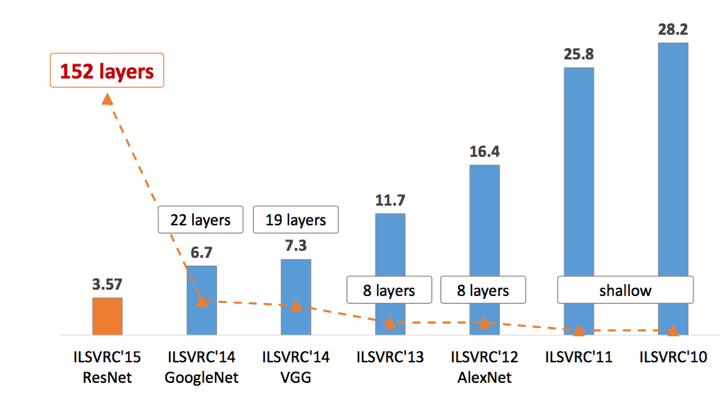
\includegraphics[height = 3in]{pics/netsCompared.png}
\caption{Comparison of performance of different image classification models in the ImageNet Large Scale Visual Recognition Competition (ILSVRC). Values indicate top-5 classification error on test datasets (how often the correct class did not appear in the top 5 outputted classes for new images).}
\label{fig:comparison}
\end{figure}
Empowered with impressive ability of feature extraction and optimization, deep convolutional neural networks has become the cornerstone of data-driven visual recognition techniques nowadays. Since AlexNet's overwhelming success in the ImageNet Large Scale Visual Recognition Competition (ILSVRC) 2012, a number of milestone model architectures have been proposed. Some common ones are described below:
\begin{itemize}
\item \textbf{AlexNet}\cite{alexnet}: Developed by Alex Krizhevsky, Ilya Sutskever and Geoff Hinton. The AlexNet significantly outperformed the second runner-up (top 5 error of 16\% compared to runner-up with 26\% error) ILSVRC challenge in 2012. It is the first work that popularized Convolutional Neural Networks in Computer Vision.

AlexNet had a similar structure to a pivotal network proposet by LeCun et al in 1998 for classifying digits\cite{lecun1998gradient}. It invokes convolutional, max pooling, and fully connected layers, also invoking ReLU activations with dropout (Figure \ref{fig:alexnet}).

\begin{figure}[!htb]
\centering
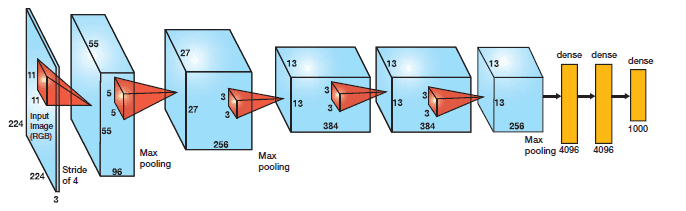
\includegraphics[height = 2in]{pics/alexnet.png}
\caption{AlexNet model architecture}
\label{fig:alexnet}
\end{figure}

\item \textbf{VGGNet}\cite{vggnet}: Proposed by Karen Simonyan and Andrew Zisserman. The VGGNet was the runner-up in ILSVRC 2014. Its main contribution was in showing that the depth of the network is a critical component for good performance. Researchers and engineers tend to design deeper rather than shallower models ever since.

VGGNet (Figure \ref{fig:vgg} is similar to AlexNet, only with more filters and more layers. The weight configuration of the VGGNet is publicly available and can be used in other applications as a feature extractor.
\begin{figure}[!htb]
\centering
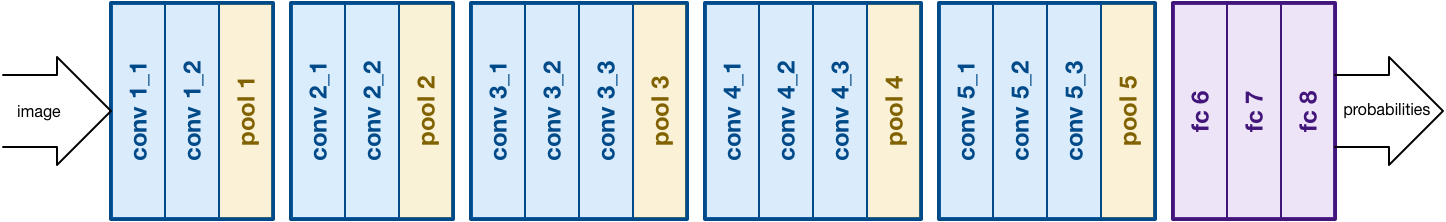
\includegraphics[height = 1in]{pics/vggnet.png}
\caption{VGGNet model architecture}
\label{fig:vgg}
\end{figure}

\item \textbf{GoogLeNet}\cite{googlenet}: As its name shows, it is authored by Szegedy \textit{et al.} from Google. GoogLeNet (Figure \ref{fig:googlenet}) was the ILSVRC 2014 winner with main contribution in developing Inception Module that dramatically reduced the number of parameters in the network. The Inception Modules (Figure \ref{fig:inception}) serve to approximate a sparse CNN with a normal dense construction. This greatly reduces the number of parameters required to optimize over (noting that many activations hence parameters will be heavily correlated). These Inception Modules massively reduced computation requirements.


\begin{figure}[H]
\centering
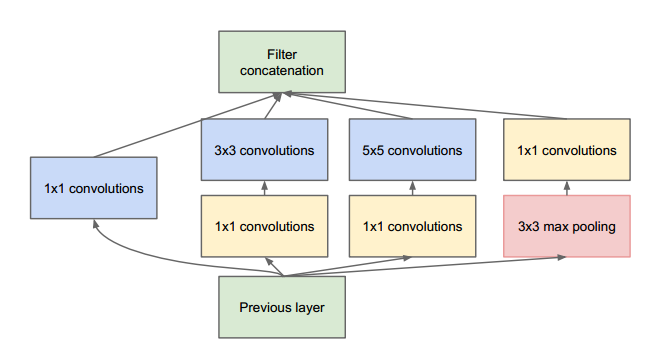
\includegraphics[height = 2.5in]{pics/InceptionModule.png}
\caption{Single Inception Module}
\label{fig:inception}
\end{figure}

\begin{figure}[!htb]
\centering
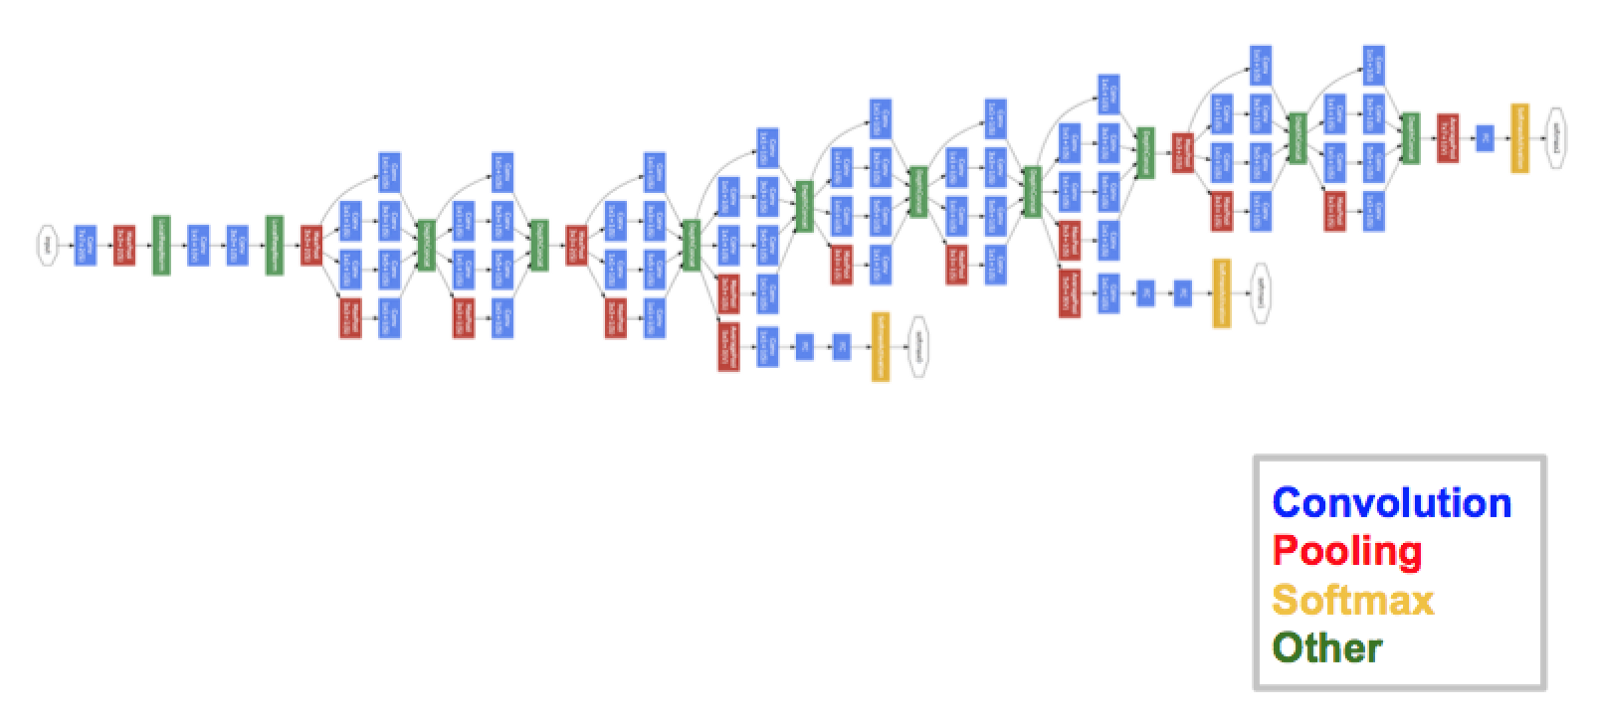
\includegraphics[scale=0.33]{pics/GoogLeNet.png}
\caption{GoogLeNet model architecture}
\label{fig:googlenet}
\end{figure}

\item \textbf{ResNet}\cite{resnet}:  Developed by Kaiming He \textit{et al.} ResNet was the winner of ILSVRC 2015. When multiple models were ensembled together, ResNet achieved a top-5 error of 3.57\%, which is astounding. ResNet implemented heavy use of batch normalization, and special skip connections now known as Residual Modules (Figure \ref{fig:residual}). CNNs have a big problem of vanishing gradients, that is, as we move farther away from our output/loss end and more towards our data, less and less gradient information gets propagated. Residual modules allay this by appending lower layers with higher ones, so that the gradients can skip operations. 

When multiple models are ensembled together, ResNet achieves a top-5 classification error of 3.57\%, which is astounding (some say this to be better-than-human accuracy). Still, the top-1 (true) classification accuracy for ResNet was roughly 80\% and has been slightly outperformed by later Inception-based models. Analysis of the evolution of these models in terms of their top-1 classification accuracy can be seen in Figure \ref{fig:top1e}.

\begin{figure}[!htb]
\centering
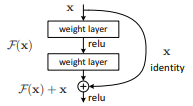
\includegraphics[height=1.5in]{pics/residual.PNG}
\caption{Residual Module\cite{resnet}}
\label{fig:residual}
\end{figure}

\begin{figure}[!htb]
\centering
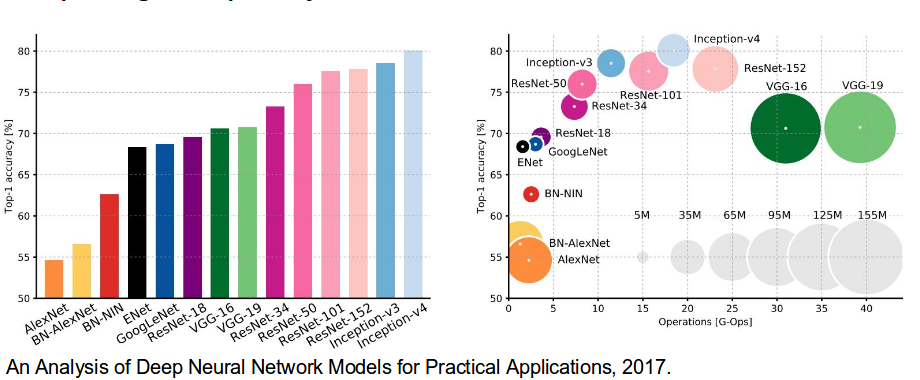
\includegraphics[height=2.5in]{pics/top1error.png}
\caption{Top-1 classification accuracy of different model architectures}
\label{fig:top1e}
\end{figure}
\end{itemize}

There also exist more model architectures proposed for specific tasks, such as YOLO\cite{yolo} and Faster R-CNN\cite{faster_rcnn} in the field of object detection and localization.

\section{Object Detection Algorithms}
\subsection{R-CNN\cite{DBLP:journals/corr/GirshickDDM13}}
The goal of R-CNN is to take in an image, and correctly identify where the main objects (via a bounding box) in the image. The network input is image and the outputs are bounding boxes + labels for each object in the image.
In summary, R-CNN is follows the steps below:
\begin{enumerate}
    \item Generate a set of proposals for bounding boxes.
    \item Run the images in the bounding boxes through a pre-trained AlexNet and finally an SVM to see what object the image in the box is.
    \item Run the box through a linear regression model to output tighter coordinates for the box once the object has been classified.
\end{enumerate}
\begin{figure}[!htb]
\centering
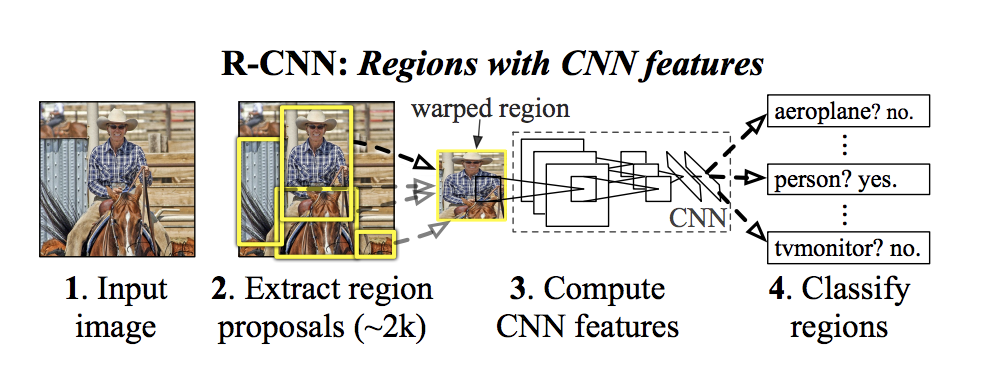
\includegraphics[height=2.5in]{pics/rcnn_intro.png}
\caption{R-CNN Algorithm}
\label{fig:rcnn1}
\end{figure}
\begin{figure}[!htb]
\centering
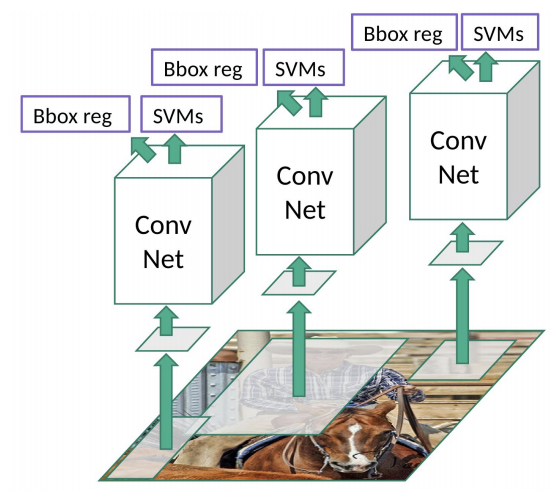
\includegraphics[height=2.5in]{pics/rcnn_intro2.png}
\caption{R-CNN Algorithm}
\label{fig:rcnn2}
\end{figure}
In terms of the bounding boxes selection, Ross Girshick et al. proposed a method\cite{DBLP:journals/corr/GirshickDDM13} where we use selective search to extract just 2000 regions from the image and he called them region proposals. Therefore, now, instead of trying to classify a huge number of regions, you can just work with 2000 regions. These 2000 region proposals are generated using the selective search algorithm which is written below.
\begin{enumerate}
    \item Generate initial sub-segmentation, we generate many candidate regions
    \item Use greedy algorithm to recursively combine similar regions into larger ones 
    \item Use the generated regions to produce the final candidate region proposals
\end{enumerate}
So far, we have seen how RCNN can be helpful for object detection. But this technique comes with its own limitations. Training an RCNN model is expensive and slow thanks to the below steps:
\begin{enumerate}
    \item Extracting 2,000 regions for each image based on selective search
    \item Extracting features using CNN for every image region. Suppose we have N images, then the number of CNN features will be N*2,000
    \item The entire process of object detection using RCNN has three models: 
    \begin{enumerate}
        \item CNN for feature extraction
        \item Linear SVM classifier for identifying objects
        \item Regression model for tightening the bounding boxes.
    \end{enumerate}
\end{enumerate}

\subsection{YOLO\cite{yolo}}
YOLO (You Only Look Once), is a network for object detection. The object detection task consists in determining the location on the image where certain objects are present, as well as classifying those objects. Previous methods for this, like R-CNN and its variations, used a pipeline to perform this task in multiple steps. This can be slow to run and also hard to optimize, because each individual component must be trained separately. YOLO, does it all with a single neural network. A image is passed through a neural network that looks similar to a normal CNN, but you get a vector of bounding boxes and class predictions in the output. The output is shown in figure \ref{fig:yolo output} and described below:
\begin{itemize}
    \item center of a bounding box (bx, by)
    \item width (bw)
    \item height (bh)
    \item value c is corresponding to a class of an object (f.e. car, traffic lights,…).
\end{itemize}
\begin{figure}[!htb]
\centering
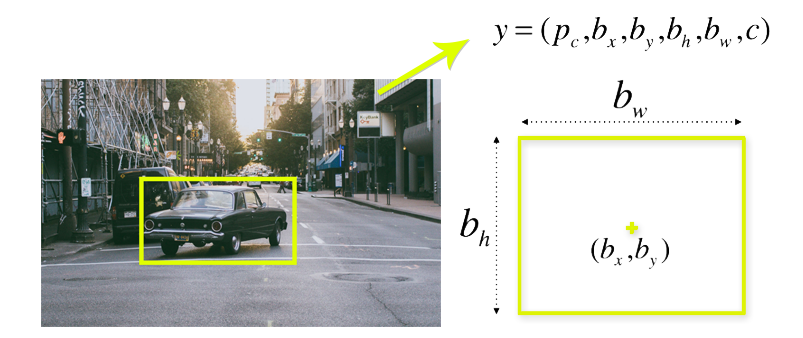
\includegraphics[height=2.5in]{pics/yolo_output.png}
\caption{YOLO Output}
\label{fig:yolo output}
\end{figure}
Firstly, we are splitting our image into cells, typically its $19 \times 19$ grid. Each cell will be responsible for predicting 5 bounding boxes in case there are more than one object in this cell. This will give us 1805 bounding boxes for an image. This is illustrated in figure \ref{fig:yolo_split}.\newline
\begin{figure}[!htb]
\centering
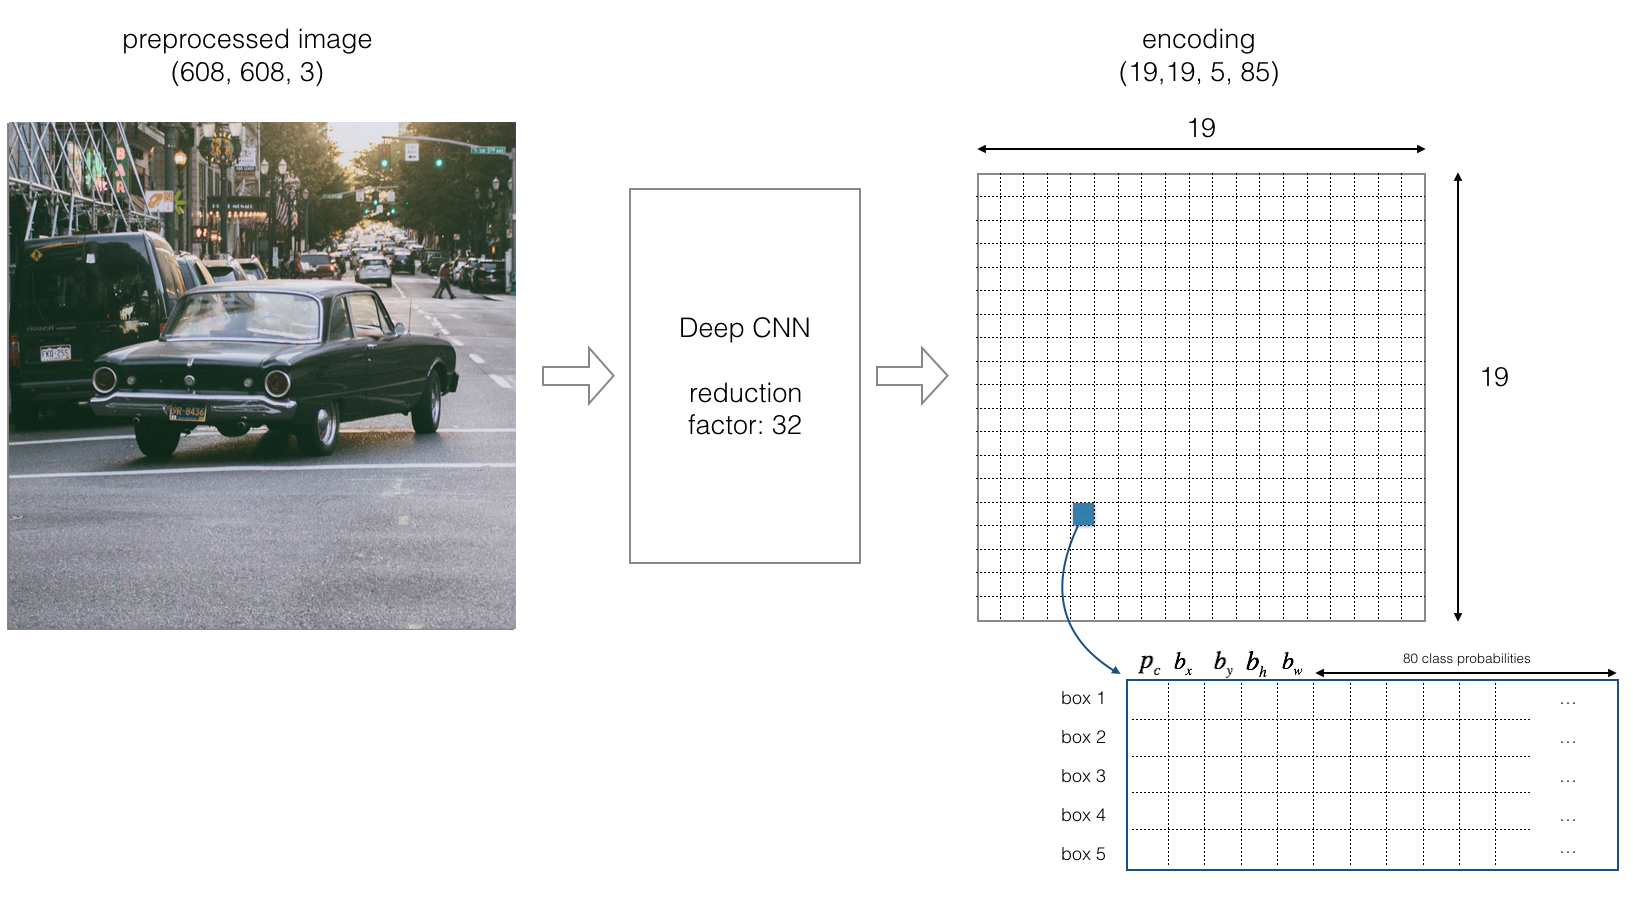
\includegraphics[height=2.5in]{pics/yolo_split.png}
\caption{YOLO: Split the Image into cells}
\label{fig:yolo_split}
\end{figure}
\noindent Then we have a deep CNN taking in the input image and spit out the output in the dimension of $(19, 19, 5, 5 + 80)$, where 80 is the number of classes. This is illustrated in figure \ref{fig:yolo_split}.\newline
Majority of those cells and boxes won’t have an object inside and this is the reason why we need to predict $p_c$. In the next step, we’re removing boxes with low object probability and bounding boxes with the highest shared area in the process called non-max suppression, which is shown in figure \ref{fig:yolo_suppression}.\newline
\begin{figure}[!htb]
\centering
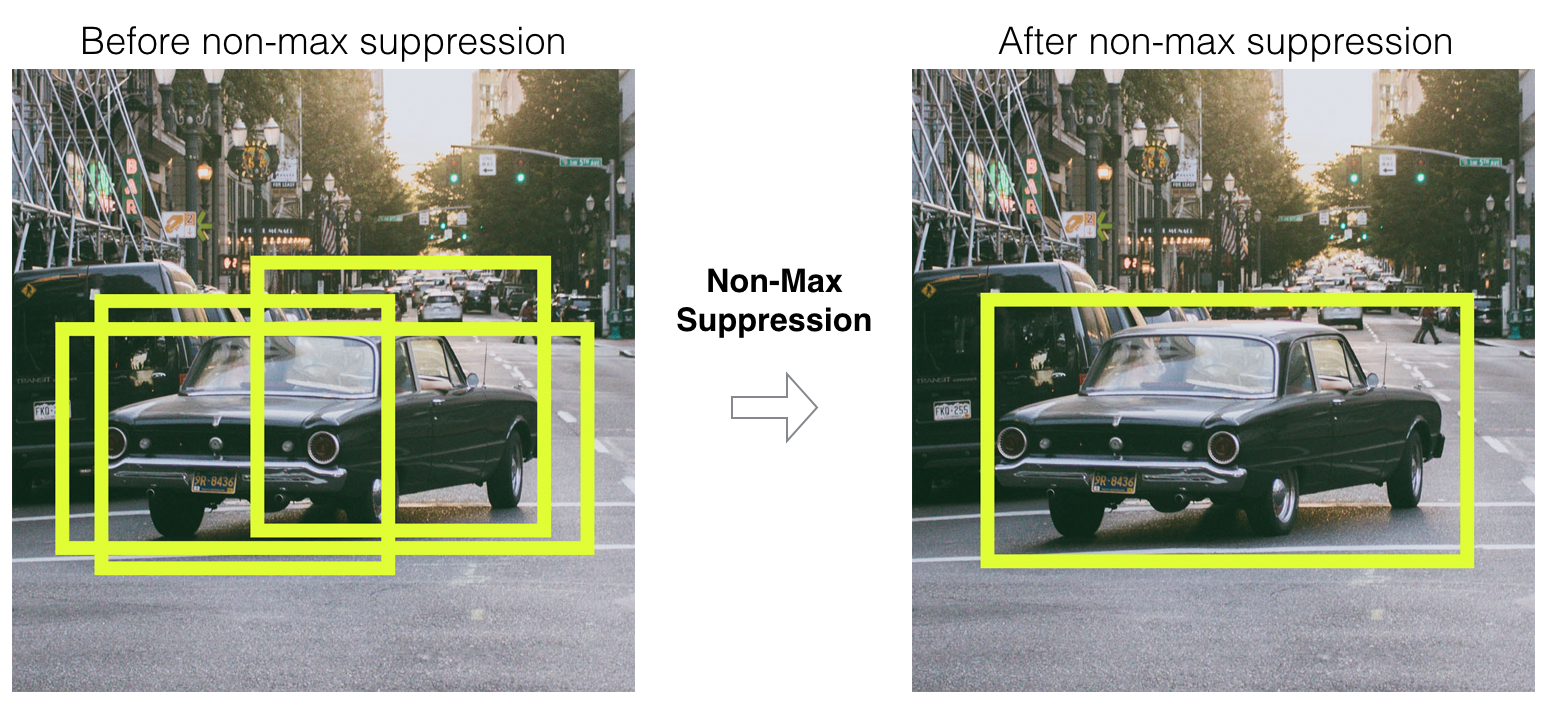
\includegraphics[height=2.5in]{pics/yolo_suppression.png}
\caption{YOLO: Non-max suppression}
\label{fig:yolo_suppression}
\end{figure}
YOLO has several advantages over classifier-based systems. It looks at the whole image at test time so its predictions are informed by global context in the image. It also makes predictions with a single network evaluation unlike systems like R-CNN which require thousands for a single image. This makes it extremely fast, more than 1000x faster than R-CNN and 100x faster than Fast R-CNN.

\section{Applications of Machine Learning in Industry}

To the reader that is being exposed to machine learning for the first time, it might be helpful to know what types of problems have been solved through the use of machine learning. Understanding the existing problem domain in which machine learning operates may inspire the reader to extend the use of methods to other domains. This section highlights some examples from recent literature.

\begin{itemize}
\item \textbf{On-board down-selection of data for spacecraft telemetry.}
One of the challenges faced by space mission designers is the volume of remote data (telemetry) that can be downlinked for examination by a human operator on the ground. Given this relatively hard physical constraint, it is useful to perform data processing on-board the spacecraft and filter the entire dataset to a (predictably) useful set of telemetry packages for downlink. The Intelligence Payload Experiment (IPEX), a CubeSat that operated on Low Earth Orbit from 2013 to 2015, utilized machine learning to accomplish this on-board autonomy task \cite{ipex}. The satellite performed on-board feature extraction and image classification over the Earth images obtained from its camera. The system was trained with a small sample of data from a suborbital flight, and classified orbital images based on its predictions of snow, water, land, haze, or cloud content. The system utilized random forest classifiers (from the TextureCam suite), which advanced previous work through enhanced analysis on spatial neighborhoods and increased regularization due to using multiple ensembles of decisions trees. This is a notable example for the use of machine learning in robotic systems with limited computational resources.

\item \textbf{Unsupervised learning algorithm to estimate scene depth and robot pose from monocular videos.} 
As studied earlier in this course, the estimation of scene depth is one of the most important outputs of computer vision in the context of autonomous robotics. Furthermore, a designer may be interested in reducing the number or complexity of sensors required to obtain a depth estimation. Zhou et al. \cite{zhou2017unsupervised} provides a framework for using unsupervised learning from a monocular video to predict depth and pose. The implementation utilizes two parallel networks (one for ego-motion modelling and another one for depth modelling), which are coupled during the calculation of the training loss, but can operate independently during test time. Empirical testing of these algorithms has demonstrated results on par, or higher in the case of pose modelling, than similar supervised methods. 

\item \textbf{Reduced dynamic models for early earthquake prediction.}
While machine learning is typically introduced in the context of computer vision and image feature extraction, it is important to remember that the framework can be used to analyze other kinds of signals. In 2018, a group of researchers at Los Alamos National Lab utilized machine learning to create a model to analyze correlations between two distinct types of geological measurements \cite{rouet2019continuous}. They constructed a machine learning model to explain readily observable data (like GPS displacement rates) as a function of deeper seismic dynamics, which typically require more sensors and time to describe accurately. To train this random forest prediction model, statistical characteristics of the seismic signal dataset were used as features and measured GPS displacement rate data as labels. According to the authors, this model could provide indirect real-time access to fault physics on deeper portions of the the Earth, thus proving useful in early detection of seismic events that could lead to a major earthquake.

\item \textbf{Enhanced catalog classification in the Mars rover image catalog.}
Mars rovers and orbiters have produced more than 22 million images of Mars over the course of history. Previously, classification of these images on public databases has been limited to a-priori knowledge of image properties (e.g. camera angle, date, time, etc.), from which the user would have to infer the set of classifiers that would produce a set of features (i.e. if an engineer is looking for images of rover wheels to analyze wheel deterioration, select images that had camera targets pointed at wheels). In 2018, Wagstaff et al. \cite{wagstaff2018deep} described the use of machine learning for feature extraction from images in databases. This resulted in expanding the set of feature class samples that would have been otherwise too costly to examine and classify through human means. Of particular interest, this model showed that a convolutional neural network trained with Earth images can be retrained to successfully classify images from Mars. It used transfer learning to adapt the AlexNet image classifier (trained on Earth dataset) via removal of the final fully connected layer, redefinition of output classes, and retraining using Caffe on the Mars image dataset.
\end{itemize}


\section{Additional Resources}
\begin{enumerate}
    \item CS231n (CNNs for Visual Recognition) class notes : http://cs231n.github.io/convolutional-networks/
    \item Live Demo - Inner Workings of a CNN : http://scs.ryerson.ca/\~aharley/vis/conv/ \\
 2D version : http://scs.ryerson.ca/\~aharley/vis/conv/flat.html
\item CS230 : https://cs230-stanford.github.io/
\item Tensorflow documentation : https://www.tensorflow.org/api\_docs/python/tf
\end{enumerate}


% References
\bibliographystyle{unsrt}
\bibliography{references}

\subsubsection*{Contributors}
Chi Zhang, Honghao Wei, Matthew Tan, Taylor Howell, Brian Jackson, Saifan Rafiq, Kevin Okseniuk

\end{document}
